\chapter{Comparison}

In the evaluation phase of the work we looked at the criteria listed below.

\begin{description}

  \item[Runtime Performance]~\\[0.1cm]
  We used each of the parsing algorithms from the implementation phase and executed them using different input files. In each instance we measured the time it took to finish the parsing process. We repeated this multiple times for each combination of parsing technique and file, so we can determine median execution times. At the end of this phase we answer~\Cref{que:speed}.

  \speed*

  \item[Memory Usage]~\\[0.1cm]
  We determined the memory usage of the different parsing implementation using \href{http://valgrind.org}{Valgrind's} heap profiler \href{http://valgrind.org/docs/manual/ms-manual.html}{Massif}.

  \item[Code Size]~\\[0.1cm]
  We counted the lines of the different implementations using the tool \href{https://github.com/AlDanial/cloc}{cloc}.

  \item[Code Complexity]~\\[0.1cm]
  For the measurement of the code complexity we determined
  \begin{itemize}
    \item the cyclomatic complexity~\cite{mccabe1976complexity}, and
    \item the Halstead complexity measures~\cite{halstead1977elements}
  \end{itemize}
  of the generated code.

  \item[Ease of Extensibility and Composability]~\\[0.1cm]
  Since there is no common way to measure either of this attributes we only looked into them from a more informal point of view. In this part of the evaluation we describe some of the features we found that hinder or enhance the extensibility and composability of the used parsing methods. At this stage we also answer~\Cref{que:closeness}:

  \closeness*

  , and argue why certain parsing libraries allow us to stay closer to the definition of the configuration language.

  \item[Error Reporting]~\\[0.1cm]
  For this subtask we created YAML input files, that contain certain errors. We then looked at what error information the parsing engines provide, and how well this information describes the given error.

\end{description}

\section{Setup}

In the following section we list the hard- and software configuration we used for the comparison.

\subsection{Hardware}

For all of the tests we used the hardware described in Table~\ref{table:benchmark_hardware}.

\begin{table}[H]
  \caption{Hardware Setup}
  \label{table:benchmark_hardware}
  \centering
  \begin{tabular}{ll}
\toprule
\multicolumn{2}{c}{MacBook Pro (Retina, 15-inch, Late 2013)}\\
\midrule
\textbf{Component} & \textbf{Description}\\
\midrule
               CPU &            i7-4960HQ\\
                   &              2.6 GHz\\
                   &        6 MB L3 Cache\\
                   &      128 MB L4 Cache\\
               RAM &                16 GB\\
                   &        1600 MHz DDR3\\
                HD &    Apple SSD SM1024F\\
                   &                 1 TB\\
\bottomrule
  \end{tabular}
\end{table}

\subsection{Software}

Table~\ref{table:benchmark_software} shows the overall software setup for the benchmarks. We tested the performance both on macOS and Linux. For the Linux setup we used the Mac version of Docker.

\begin{table}[H]
    \newcommand{\YAEP}{{\href{https://github.com/vnmakarov/yaep/commit/550de4cc5600d5f6109c7ebcfbacec51bf80d8d3}{YAEP 550de4cc}}}
    \caption{Software Setup}
    \label{table:benchmark_software}
    \begin{subtable}[t]{.45\linewidth}
      \centering
        \caption{Mac Setup}
        \label{table:benchmark_mac}
        \begin{tabular}{ll}
\toprule
\textbf{Component} & \textbf{Description}\\
\midrule
                OS &        macOS 10.14.5\\
                   &                     \\
\midrule
          Compiler &          Clang 8.0.0\\
        Generators &          ANTLR 4.7.2\\
                   &          Bison 3.4.1\\
         Libraries &       yaml-cpp 0.6.2\\
                   &                \YAEP\\
                   &          PEGTL 2.8.0\\
    Other Software &         CMake 3.14.4\\
                   &          Ninja 1.9.0\\
                   &      hyperfine 1.5.0\\
\bottomrule
        \end{tabular}
    \end{subtable}
    \begin{subtable}[t]{.45\linewidth}
      \centering
        \caption{Linux Setup}
        \label{table:benchmark_docker}
        \begin{tabular}{ll}
\toprule
\textbf{Component} &      \textbf{Description}\\
\midrule
            Docker &    18.09.2, build 6247962\\
        Base Image & Debian sid (sid-20190506)\\
\midrule
         Compilers &     Clang 6.0.1/GCC 8.3.0\\
        Generators &               ANTLR 4.7.2\\
                   &               Bison 3.3.2\\
         Libraries &            yaml-cpp 0.6.2\\
                   &                     \YAEP\\
                   &               PEGTL 2.7.1\\
    Other Software &              CMake 3.13.4\\
                   &               Ninja 1.8.2\\
                   &           hyperfine 1.5.0\\
\bottomrule
        \end{tabular}
    \end{subtable}
\end{table}

\subsection{Build Setup}

The following list shows the \href{https://cmake.org}{CMake} options that we used for all comparisons:

\begin{itemize}
  \item \sh{-GNinja}
  \item \sh{-DPLUGINS=ALL}
\end{itemize}

. For

\begin{itemize}
  \item the runtime performance benchmark, described in section “\nameref{sec:run_time_performance}”, and
  \item the heap memory usage comparison, described in section “\nameref{sec:memory_usage}”
\end{itemize}

we built Elektra using the following \href{https://cmake.org}{CMake} options:

\begin{itemize}
  \item \sh{-DCMAKE_BUILD_TYPE=Release}
  \item \sh{-DENABLE_LOGGER=OFF}
  \item \sh{-DENABLE_DEBUG=OFF}
\end{itemize}

.

\section{Runtime Performance}
\label{sec:run_time_performance}

\newcommand{\FilePluginGetSet}{{%
\href{https://master.libelektra.org/benchmarks/plugingetset.c}%
{\sh{benchmark_plugingetset}}%
}}
\newcommand{\FileBenchmarkYAML}{{%
\href{https://master.libelektra.org/scripts/benchmark-yaml.in}%
{\sh{benchmark-yaml}}%
}}
\newcommand{\FileBenchmarkRuntime}{{%
\href{https://github.com/sanssecours/rawdata/blob/⏱/YAML/Scripts/benchmark-runtime}%
{\sh{benchmark-runtime}}%
}}

To compare the runtime performance we used the C application \FilePluginGetSet{} that opens an Elektra plugin using a specific configuration file. For the whole benchmark process we created a Bash script, called \FileBenchmarkYAML{}, that uses the benchmarking tool \href{https://github.com/sharkdp/hyperfine}{\sh{hyperfine}} to call \FilePluginGetSet{} using different YAML plugins. Figure~\ref{fig:benchmark} shows a diagram of this setup.

For the measurement we use \href{https://github.com/sharkdp/hyperfine}{\sh{hyperfine}}, sine this tool

\begin{enumerate}
  \item automatically determines how often it should call \FilePluginGetSet{} for meaningful measurement results,
  \item shows us when it is time to redo the benchmark, by informing us about statistical outliers, and
  \item prints important statistical data such as the mean runtime and the standard derivation
\end{enumerate}

.

To make sure we repeat the benchmark every time \href{https://github.com/sharkdp/hyperfine}{\sh{hyperfine}} reporte statistical outliers we created the Shell script \FileBenchmarkRuntime{}. This script calls \FileBenchmarkYAML{} for every input file and repeats a benchmark, until \href{https://github.com/sharkdp/hyperfine}{\sh{hyperfine}} does not report any warning. The script \FileBenchmarkRuntime{} \emph{does} ignore warnings about runtimes under 5 milliseconds though, since \FilePluginGetSet{} might take less execution time for YAML files that only contain a few lines.

\begin{figure}[H]
  \centering
    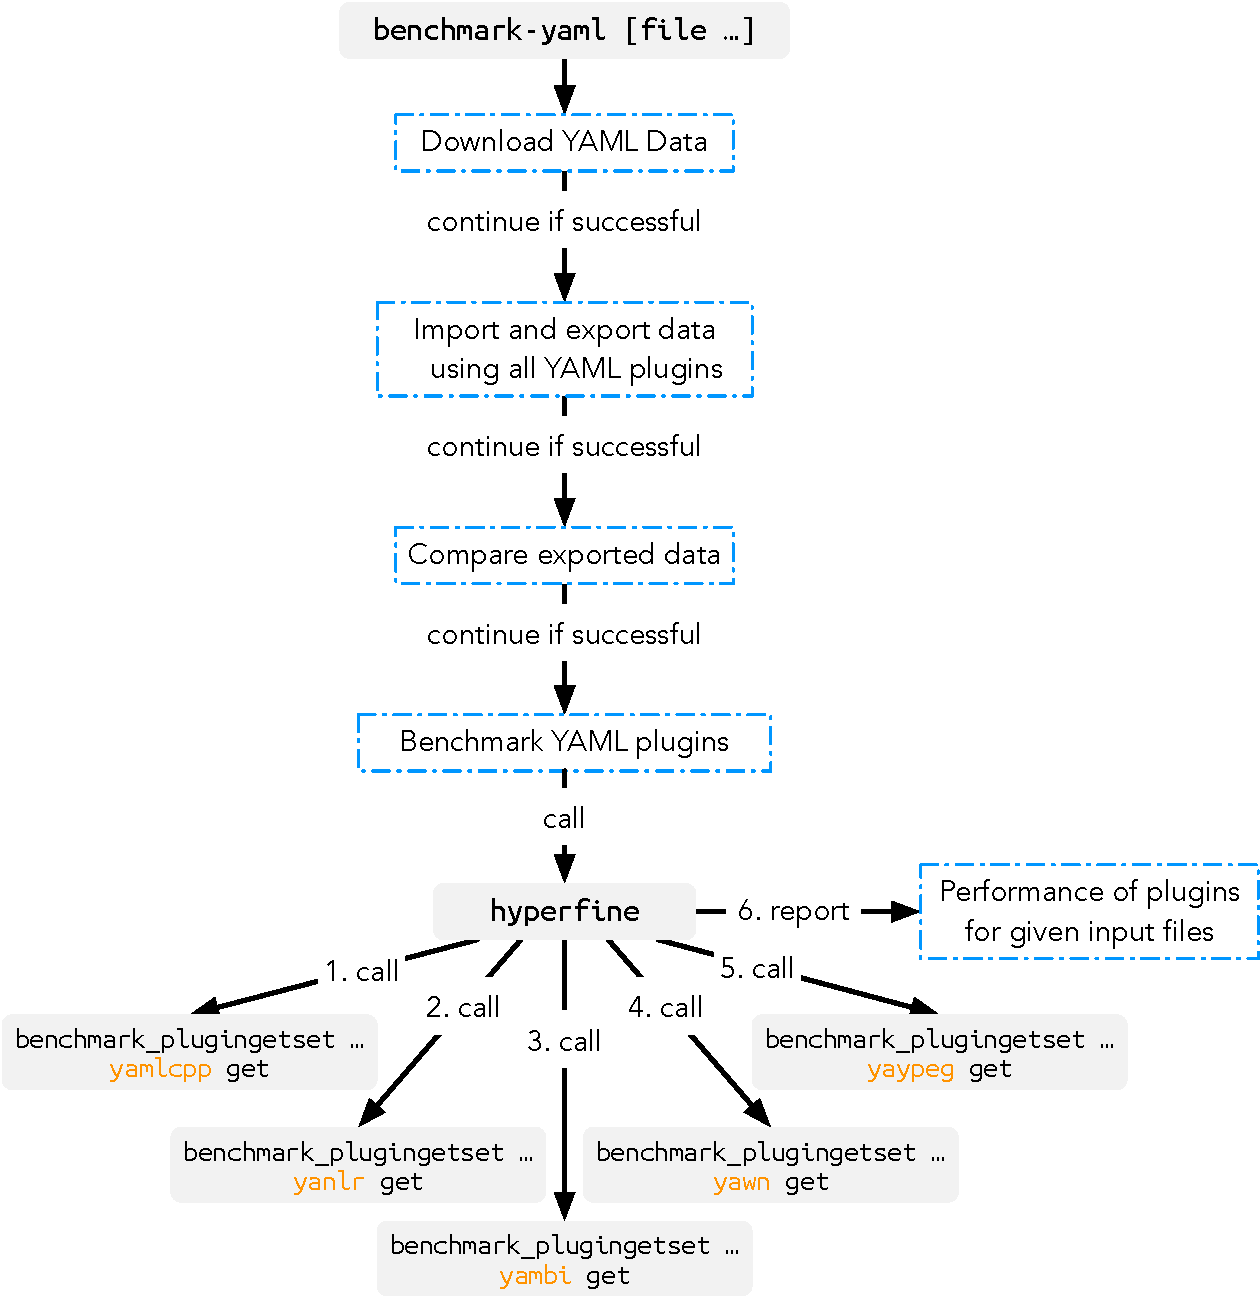
\includegraphics[width=0.9\textwidth]{Benchmark}
  \caption{The diagram above shows the basic sequence of steps to measure the performance of the YAML plugins.}
  \label{fig:benchmark}
\end{figure}

\subsection{Input}

\newcommand{\URLKeyFramesJSON}{https://master.libelektra.org/src/plugins/yajl/yajl/keyframes_complex.json}

\newcommand{\FileKeyFrames}{{%
\href{https://github.com/ElektraInitiative/rawdata/tree/master/YAML/Input/keyframes.yaml}%
{\code{keyframes.yaml}}%
}}
\newcommand{\FileCombined}{{%
\href{https://github.com/ElektraInitiative/rawdata/tree/master/YAML/Input/combined.yaml}%
{\code{combined.yaml}}%
}}
\newcommand{\FileGenerated}{{%
\href{https://github.com/ElektraInitiative/rawdata/tree/master/YAML/Input/generated.yaml}%
{\code{generated.yaml}}%
}}
\newcommand{\FileGeneratedHundredThousand}{{%
\href{https://github.com/ElektraInitiative/rawdata/tree/master/YAML/Input/generated_100000.yaml}%
{\code{generated\_100000.yaml}}%
}}
\newcommand{\FileGenerateYAML}{{%
\href{https://master.libelektra.org/scripts/generate-yaml}%
{\sh{generate-yaml}}%
}}
\newcommand{\FileCutInput}{{%
\href{https://github.com/ElektraInitiative/rawdata/tree/master/YAML/Scripts/cut_input}%
{\sh{cut_input}}%
}}

As the first input for the benchmark we used a \href{\URLKeyFramesJSON}{JSON configuration file} of the \href{https://www.libelektra.org/plugins/yajl}{YAJL plugin} that we converted to block syntax using the \href{https://www.libelektra.org/plugins/yamlcpp}{YAML CPP} plugin. We then modified the exported data by removing all \yaml{!<!elektra/meta>} tags, which are not supported by the other YAML plugins. We call the resulting file \FileKeyFrames{} in the remainder of the thesis. This file and all other data of the benchmark is available here:

\begin{leftbar}
  \url{https://github.com/ElektraInitiative/rawdata/tree/master/YAML}
\end{leftbar}

. For another input file called \FileCombined{} we copy and pasted parts of test data and various other YAML files in Elektra’s repository into a single file. While the file content is nonsensical, it should at least contains a mix of YAML data that covers most of the code paths of the YAML plugins.

Since both of these files are relatively small, \FileKeyFrames{} contains 218 lines, while \FileCombined{} contains 152 lines, we also generated data using a Python script that we called \FileGenerateYAML{}. This script generates YAML maps using \href{https://en.wikipedia.org/wiki/Universally_unique_identifier}{\glspl{UUID}} as scalar keys and values. For the YAML scalars the script randomly selects one of the three flow scalar styles:

\begin{itemize}
  \item single quoted scalar,
  \item double quoted scalar, or
  \item plain scalar
\end{itemize}

. This always works since \glspl{UUID} contain no character sequence that has special meaning according to the YAML specification. Using this method we generated two files:

\begin{itemize}
  \item \FileGenerated{} that contains 10 000 lines, and

  \item \FileGeneratedHundredThousand{} that contains 100 000 lines
\end{itemize}

. We also created another script called \FileCutInput{} to generate additional smaller input files that contain the first 50000, 10000, 5000, 1000, 500, 100, 50, 10, 5 and 1 lines of \FileGeneratedHundredThousand{}.

\subsection{Results}

The graphs in this section show the results of the benchmark for different input files. The basis of all results is \href{https://github.com/ElektraInitiative/libelektra/commit/54a4c0194946917b7d093e0777f465619b2f3d6f}{commit 54a4c019} of Elektra’s code base.

\begin{figure}[H]
  \begin{bchart}[max=30, width=0.8\textwidth, unit=ms]
    \bcbar[text=17.7 ± 0.7, value=macOS, color=orange]{17.7}
    \bcbar[text=25.5 ± 3.5, value=Linux/GCC, color=orange]{25.5}
    \bcbar[text=24.2 ± 2.9, value=Linux/Clang, color=orange]{24.2}

    \bcbar[text=15.8 ± 0.8, value=macOS, color=DarkYellow]{15.8}
    \bcbar[text=27.3 ± 2.3, value=Linux/GCC, color=DarkYellow]{27.3}
    \bcbar[text=25.8 ± 1.6, value=Linux/Clang, color=DarkYellow]{25.8}

    \bcbar[text=18.7 ± 1, value=macOS, color=Turquoise3]{18.7}
    \bcbar[text=20.1 ± 1.8, value=Linux/GCC, color=Turquoise3]{20.1}
    \bcbar[text=20.1 ± 1.6, value=Linux/Clang, color=Turquoise3]{20.1}

    \bcbar[text=13.8 ± 0.7, value=macOS, color=Aqua]{15.4}
    \bcbar[text=21.6 ± 1.8, value=Linux/GCC, color=Aqua]{21.6}
    \bcbar[text=19.8 ± 1.1, value=Linux/Clang, color=Aqua]{19.8}

    \bcbar[text=23.8 ± 1, value=macOS, color=DarkOrchid]{23.8}
    \bcbar[text=22.8 ± 2.2, value=Linux/GCC, color=DarkOrchid]{22.8}
    \bcbar[text=22.3 ± 2.1, value=Linux/Clang, color=DarkOrchid]{22.3}
  \end{bchart}
  \begin{center}
  \vspace{-0.5cm}
    \tikzcircle{orange} YAML CPP ~~
    \tikzcircle{DarkYellow} Yan LR ~~
    \tikzcircle{Turquoise3} YAMBi ~~
    \tikzcircle{Aqua} YAwn ~~
    \tikzcircle{DarkOrchid} YAy PEG
  \vspace{-0.5cm}
  \end{center}
  \caption{This bar chart shows the run time of the plugins for the input \FileKeyFrames{}.}
  \label{fig:benchmark_keyframes}
\end{figure}

\begin{figure}[H]
  \begin{bchart}[max=35, width=0.8\textwidth, unit=ms]
    \bcbar[text=12.3 ± 0.9, value=macOS, color=orange]{12.3}
    \bcbar[text=24.1 ± 2.7, value=Linux/GCC, color=orange]{24.1}
    \bcbar[text=22.2 ± 2.5, value=Linux/Clang, color=orange]{22.2}

    \bcbar[text=9.3 ± 0.5, value=macOS, color=DarkYellow]{9.3}
    \bcbar[text=24.6 ± 1.5, value=Linux/GCC, color=DarkYellow]{24.6}
    \bcbar[text=22.8 ± 1.5, value=Linux/Clang, color=DarkYellow]{22.8}

    \bcbar[text=11.9 ± 0.8, value=macOS, color=Turquoise3]{11.9}
    \bcbar[text=19.4 ± 1.4, value=Linux/GCC, color=Turquoise3]{19.4}
    \bcbar[text=18.9 ± 1.9, value=Linux/Clang, color=Turquoise3]{18.9}

    \bcbar[text=8.2 ± 0.6, value=macOS, color=Aqua]{8.2}
    \bcbar[text=20.2 ± 1.9, value=Linux/GCC, color=Aqua]{20.2}
    \bcbar[text=21.5 ± 4.2, value=Linux/Clang, color=Aqua]{21.5}

    \bcbar[text=14.3 ± 0.7, value=macOS, color=DarkOrchid]{14.3}
    \bcbar[text=20.3 ± 1.8, value=Linux/GCC, color=DarkOrchid]{20.3}
    \bcbar[text=19.7 ± 3.2, value=Linux/Clang, color=DarkOrchid]{19.7}
  \end{bchart}
  \begin{center}
  \vspace{-0.5cm}
    \tikzcircle{orange} YAML CPP ~~
    \tikzcircle{DarkYellow} Yan LR ~~
    \tikzcircle{Turquoise3} YAMBi ~~
    \tikzcircle{Aqua} YAwn ~~
    \tikzcircle{DarkOrchid} YAy PEG
  \vspace{-0.5cm}
  \end{center}
  \caption{This bar chart shows the run time of the plugins for the input \FileCombined{}.}
  \label{fig:benchmark_combined}
\end{figure}

\begin{figure}[H]
  \begin{bchart}[max=385, width=0.8\textwidth, unit=ms]
    \bcbar[text=239.5 ± 4.3, value=macOS, color=orange]{239.5}
    \bcbar[text=139.4 ± 2.8, value=Linux/GCC, color=orange]{139.4}
    \bcbar[text=137.3 ± 11.8, value=Linux/Clang, color=orange]{137.3}

    \bcbar[text=119.9 ± 1.1, value=macOS, color=DarkYellow]{119.9}
    \bcbar[text=123.7 ± 2.2, value=Linux/GCC, color=DarkYellow]{123.7}
    \bcbar[text=124.5 ± 5.2, value=Linux/Clang, color=DarkYellow]{124.5}

    \bcbar[text=174.8 ± 1.7, value=macOS, color=Turquoise3]{174.8}
    \bcbar[text=65 ± 2.4, value=Linux/GCC, color=Turquoise3]{65}
    \bcbar[text=64.8 ± 2.5, value=Linux/Clang, color=Turquoise3]{64.8}

    \bcbar[text=73.6 ± 1, value=macOS, color=Aqua]{73.6}
    \bcbar[text=77.3 ± 2.6, value=Linux/GCC, color=Aqua]{77.3}
    \bcbar[text=74.9 ± 3.1, value=Linux/Clang, color=Aqua]{74.9}

    \bcbar[text=363.2 ± 2, value=macOS, color=DarkOrchid]{363.2}
    \bcbar[text=156.8 ± 5.7, value=Linux/GCC, color=DarkOrchid]{156.8}
    \bcbar[text=161.1 ± 7.5, value=Linux/Clang, color=DarkOrchid]{161.1}
  \end{bchart}
  \begin{center}
  \vspace{-0.5cm}
    \tikzcircle{orange} YAML CPP ~~
    \tikzcircle{DarkYellow} Yan LR ~~
    \tikzcircle{Turquoise3} YAMBi ~~
    \tikzcircle{Aqua} YAwn ~~
    \tikzcircle{DarkOrchid} YAy PEG
  \vspace{-0.5cm}
  \end{center}
  \caption{This bar chart shows the run time of the plugins for the input \FileGenerated{}.}
  \label{fig:benchmark_generated}
\end{figure}

\begin{figure}[H]
  \centering
    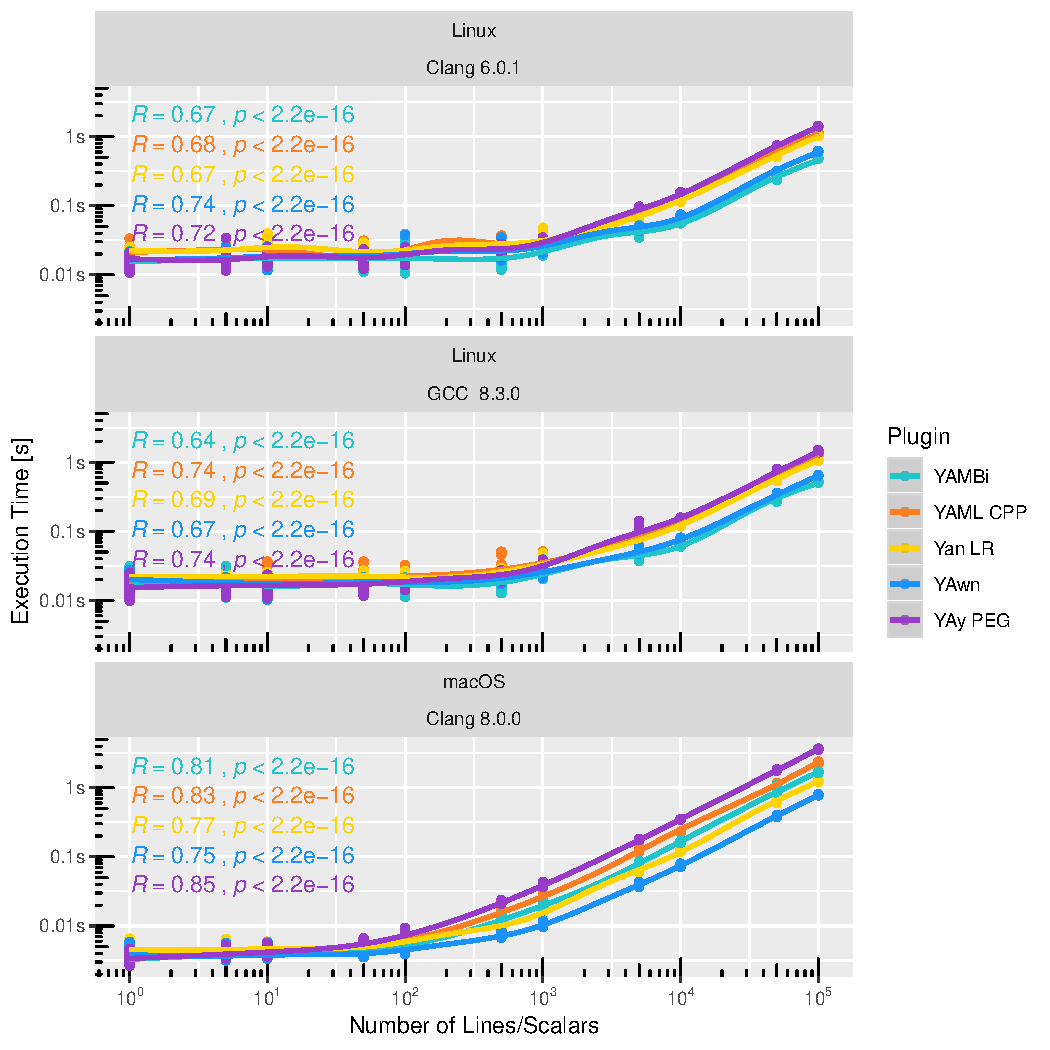
\includegraphics[width=\textwidth]{BenchmarkResultRuntime}
  \caption{The diagrams above show the runtime of the plugins for the input file \FileGeneratedHundredThousand{} and other files that contain only the first $n$ number of lines of this file.}
  \label{fig:benchmark_results_generated}
\end{figure}

\subsection{Analysis}

If we look at Figure~\ref{fig:benchmark_results_generated} we see that the runtime seems to grow linearly after a certain number of input lines. To verify this we hypothesis we removed all samples with a line length smaller than 1000. Figure~\ref{fig:benchmark_results_generated_above_1000} shows the result.

\begin{figure}[H]
  \centering
    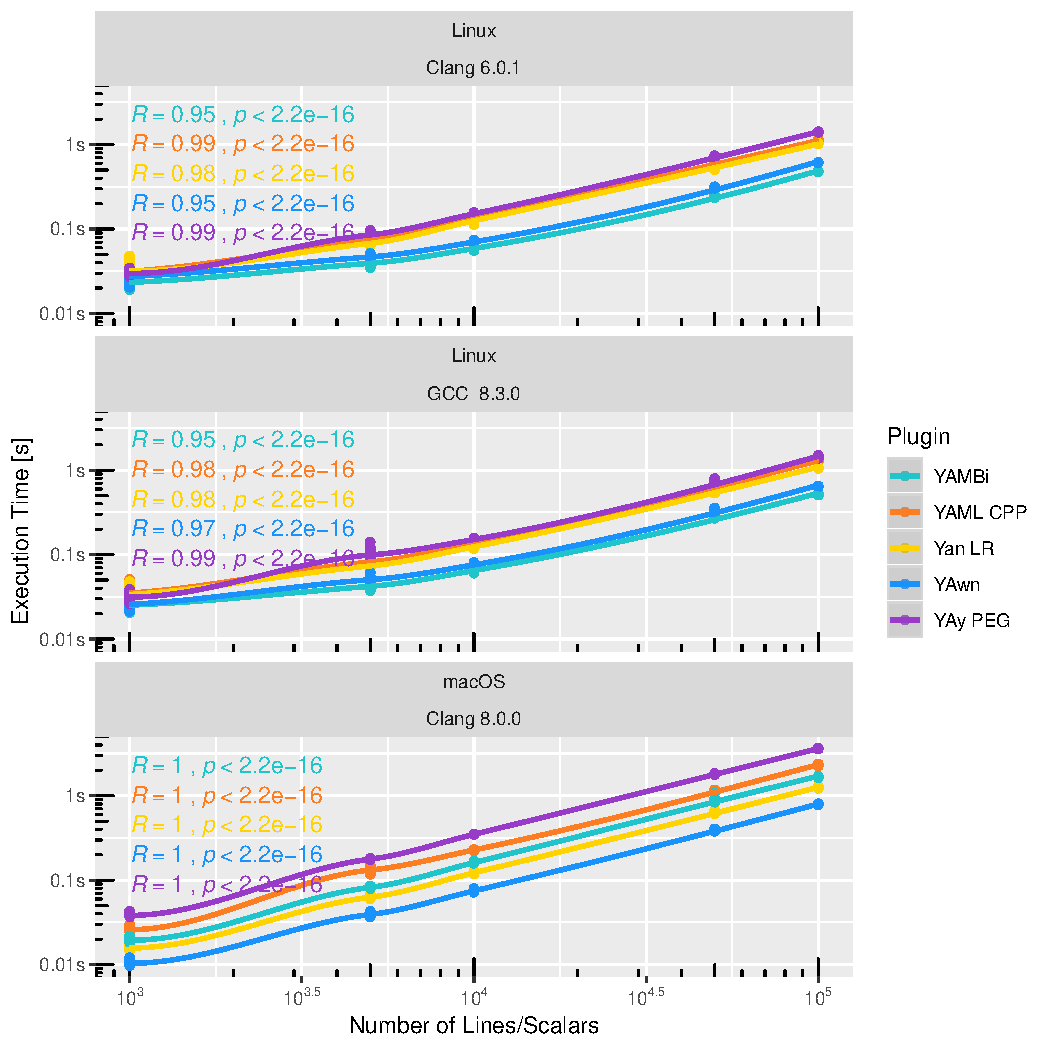
\includegraphics[width=\textwidth]{BenchmarkResultRuntimeAbove1000}
  \caption{The diagrams above shows that the runtime for the first lines of the file \FileGeneratedHundredThousand{} almost certainly grows linearly.}
  \label{fig:benchmark_results_generated_above_1000}
\end{figure}

From the correlation coefficients ($R$) of $0.95$ and higher we deduce that the runtime for all plugins almost certainly grows linearly. This means that the approximate runtime of the plugins should be the same. Now it is time to answer \Cref{que:speed}.

\speed*

The runtime of a non-backtracking recursive descent parser for an LL(1) grammar, as used by YAML CPP, should be $O(n)$. According to the literature the upper boundary for the runtime of

\begin{itemize}
  \item \gls{ALL(*)}, used by Yan LR, is $O(n⁴)$, but the algorithm often performs linearly~\cite[p. 1]{parr2014adaptive},
  \item LALR, used by YAMBi, is $O(n)$~\cite{baxter2017runtime},
  \item an Early parser, used by YAwn, is $O(n²)$ for unambiguous grammars~\cite[p. 145]{hopcroft1969formal},
  \item a general PEG parsers, as used by YAy PEG, is exponential~\cite[p. 1]{moss2014derivatives} ($O(cⁿ)$) and for PEG parsers that use memoization is $O(n)$~\cite{ford2002packrat}
\end{itemize}

. We now compare the theoretic runtimes with the measured runtimes shown in Figure~\ref{fig:benchmark_results_generated_above_1000}. The text below lists some of our observations.

\begin{itemize}
  \item The deterministic (aka non-backtracking) parsers (YAML CPP, YAMBi) show the expected linear behavior.

  \item Yan LR also executes in linear time for the input. This is probably the result of the relatively simple grammar used by the parser. At least for all our input and test files we also checked that the grammar works with the simpler, but faster \gls{SLL(*)} strategy. This was indeed the case.

  \item YAwn also shows the linear behavior, even though \href{https://github.com/vnmakarov/yaep}{\gls{YAEP}} \href{https://github.com/vnmakarov/yaep/issues/24}{does not implement \citeauthor{leo1991general}’s optimization}~\cite{leo1991general} that makes sure that the algorithm runs in linear time for every LR(k) grammar.

  \item Even YAy PEG’s backtracking parser without memoization show linear behavior. This also corroborates the statement by \citeauthor{hirsch2016memo}, one of PEGTL’s authors statement about memoization~\cite{hirsch2016memo}, quoted below.

  \begin{quote}
     …in practice packrat parsers often perform worse than simple recursive descent parsers despite being in a better time complexity class.
  \end{quote}

\end{itemize}

Figure~\ref{fig:benchmark_generated} shows that the constant difference between the linear runtimes can be relatively high. For example on macOS, the fastest plugin YAwn is nearly five times faster than the slowest plugin YAy PEG for the file \FileGenerated{}:

\begin{equation}
  \frac{363.2\text{ms}}{73.6\text{ms}} ≅ 4.93
  \label{eq:benchmark_difference}
\end{equation}

. Other interesting observations concerning the runtime are listed below.

\begin{enumerate}
  \item The difference between the runtime of the fastest and slowest plugins for large files is nearly twice as large on macOS.

  \item The OS seems to play a much more important role, than the compiler for all of the used YAML libraries.

  \item While Yan LR and YAwn perform similarly on macOS and Linux, the difference between YAML CPP, YAMBi and YAy PEG on both operating systems can be quite significant.
\end{enumerate}

Since the runtime of the plugins is quite different on the two benchmarked operating systems we also determined mean of the mean values for the file \FileGenerated{}. We use a weight of

\begin{itemize}
  \item $0.5$ for the combination macOS/Clang,
  \item $0.25$ for the combination Linux/Clang, and
  \item $0.25$ for the combination Linux/GCC
\end{itemize}

and obtain the formula:

\begin{equation}
  \overline{t} = 0.5  · \overline{t}_{\text{macOS/Clang}} +
                 0.25 · \overline{t}_{\text{Linux/GCC}} +
                 0.25 · \overline{t}_{\text{Linux/Clang}}
  \label{eq:benchmark_generated_mean}
\end{equation}

. Figure \ref{fig:benchmark_generated_mean} shows a bar graph with the result of this calculation.

\begin{figure}[H]
  \begin{bchart}[max=300, width=0.8\textwidth, unit=ms]

    \bcbar[text=188.9, value=, color=orange]{188.9}

    \bcbar[text=122, value=, color=DarkYellow]{122}

    \bcbar[text=119.9, value=, color=Turquoise3]{119.9}

    \bcbar[text=74.9, value=, color=Aqua]{74.9}

    \bcbar[text=261, value=, color=DarkOrchid]{261}
  \end{bchart}
  \begin{center}
  \vspace{-0.5cm}
    \tikzcircle{orange} YAML CPP ~~
    \tikzcircle{DarkYellow} Yan LR ~~
    \tikzcircle{Turquoise3} YAMBi ~~
    \tikzcircle{Aqua} YAwn ~~
    \tikzcircle{DarkOrchid} YAy PEG
  \vspace{-0.5cm}
  \end{center}
  \caption{This bar chart shows the mean of the mean run times of the plugins according to Equation~\ref{eq:benchmark_generated_mean} for the input \FileGenerated{}.}
  \label{fig:benchmark_generated_mean}
\end{figure}

\subsection{Conclusion}

We determined with a high confidence that all of the YAML plugins show a linear runtime behavior (see Figure~\ref{fig:benchmark_results_generated_above_1000}). This puts the plugin into the same computational complexity class. The constant difference between the runtime can still be relatively high though, as we can see in Equation~\ref{eq:benchmark_difference}.

The fastest plugin according to the mean of the mean runtimes (see Figure~\ref{fig:benchmark_generated_mean}) is YAwn, if we weigh the results of the two tested operating systems equally. This is interesting, since \citeauthor{earley1970efficient} himself mentions in his dissertation~\cite[p. 122]{earley1970efficient} that his parsing technique was too slow for practical use at the time, as you can see in the quote below.

\begin{quote}
  First we ask, what impact will our algorithm have on the parsing done in production compilers for existing programming languages? The answer is, practically none. Production compilers require guessing time proportional to n with a fairly low coefficient of n.
\end{quote}

Yan LR and YAMBi showed the second best runtimes, and were about $1.6$ times slower than YAwn. YAML CPP, which was, according to the results of Figure~\ref{fig:benchmark_generated_mean}, about $2.5$ times slower than Yawn takes the second to last place. Yay PEG was the slowest plugin on both tested operating systems, and is about $3.5$ times slower than the fastest plugin according to Figure~\ref{fig:benchmark_generated_mean}.

\section{Memory Usage}
\label{sec:memory_usage}

\newcommand{\FileBenchmarkMemory}{{%
\href{https://github.com/sanssecours/rawdata/blob/⏱/YAML/Scripts/benchmark-memory}%
{\sh{benchmark-memory}}%
}}

We measured the heap memory usage with the heap profiler \href{http://valgrind.org/docs/manual/ms-manual.html}{Massif}. Most of the other setup is similar to the one we used for the runtime benchmark, described in the section “\nameref{sec:run_time_performance}”. We still use the the C application \FilePluginGetSet{} to execute the plugins. The input files are also the same as before.

This time we do not need to determine the mean value of the results. Massif always produces the same output on the same hardware/software combination, since it runs the instrumented program \FilePluginGetSet{} on a “synthetic CPU”~\cite{valgrind2019core}.

To automate the process of measuring the memory usage for the different input files, we created a Shell script called \FileBenchmarkMemory{}. We only benchmarked the memory usage on Linux, since Massif did not support macOS 10.14 at the time we executed the benchmark script.

\subsection{Results}

The graphs in this section show the results of the memory benchmark for different input files. The basis of all results is \href{https://github.com/ElektraInitiative/libelektra/commit/ea418f177a5e2707f59f61b5e130a596abdd1c56}{commit ea418f17} of Elektra’s code base.

\begin{figure}[H]
  \begin{bchart}[max=25, width=0.8\textwidth, unit=MB]
    \bcbar[text=17.5, value=Linux/GCC, color=orange]{17.5}
    \bcbar[text=18.3, value=Linux/Clang, color=orange]{18.3}

    \bcbar[text=23.8, value=Linux/GCC, color=DarkYellow]{23.8}
    \bcbar[text=23.8, value=Linux/Clang, color=DarkYellow]{23.8}

    \bcbar[text=10.4, value=Linux/GCC, color=Turquoise3]{10.4}
    \bcbar[text=10.1, value=Linux/Clang, color=Turquoise3]{10.1}

    \bcbar[text=9, value=Linux/GCC, color=Aqua]{9}
    \bcbar[text=8.8, value=Linux/Clang, color=Aqua]{8.8}

    \bcbar[text=22.8, value=Linux/GCC, color=DarkOrchid]{22.8}
    \bcbar[text=23.1, value=Linux/Clang, color=DarkOrchid]{23.1}
  \end{bchart}
  \begin{center}
  \vspace{-0.5cm}
    \tikzcircle{orange} YAML CPP ~~
    \tikzcircle{DarkYellow} Yan LR ~~
    \tikzcircle{Turquoise3} YAMBi ~~
    \tikzcircle{Aqua} YAwn ~~
    \tikzcircle{DarkOrchid} YAy PEG
  \vspace{-0.5cm}
  \end{center}
  \caption{This bar chart shows the peak heap memory usage of the plugins for the input \FileKeyFrames{}.}
  \label{fig:benchmark_memory_keyframes}
\end{figure}

\begin{figure}[H]
  \begin{bchart}[max=20, width=0.8\textwidth, unit=MB]
    \bcbar[text=12.6, value=Linux/GCC, color=orange]{12.6}
    \bcbar[text=12.9, value=Linux/Clang, color=orange]{12.9}

    \bcbar[text=17.5, value=Linux/GCC, color=DarkYellow]{17.5}
    \bcbar[text=17.4, value=Linux/Clang, color=DarkYellow]{17.4}

    \bcbar[text=7.7, value=Linux/GCC, color=Turquoise3]{7.7}
    \bcbar[text=7.6, value=Linux/Clang, color=Turquoise3]{7.6}

    \bcbar[text=7.9, value=Linux/GCC, color=Aqua]{7.9}
    \bcbar[text=7.8, value=Linux/Clang, color=Aqua]{7.8}

    \bcbar[text=14.8, value=Linux/GCC, color=DarkOrchid]{14.8}
    \bcbar[text=14.8, value=Linux/Clang, color=DarkOrchid]{14.8}
  \end{bchart}
  \begin{center}
  \vspace{-0.5cm}
    \tikzcircle{orange} YAML CPP ~~
    \tikzcircle{DarkYellow} Yan LR ~~
    \tikzcircle{Turquoise3} YAMBi ~~
    \tikzcircle{Aqua} YAwn ~~
    \tikzcircle{DarkOrchid} YAy PEG
  \vspace{-0.5cm}
  \end{center}
  \caption{This bar chart shows the peak heap memory usage of the plugins for the input \FileCombined{}.}
  \label{fig:benchmark_memory_combined}
\end{figure}

\begin{figure}[H]
  \begin{bchart}[max=700, width=0.8\textwidth, unit=MB]
    \bcbar[text=526.4, value=Linux/GCC, color=orange]{526.4}
    \bcbar[text=555, value=Linux/Clang, color=orange]{555}

    \bcbar[text=483.5, value=Linux/GCC, color=DarkYellow]{483.5}
    \bcbar[text=480.9, value=Linux/Clang, color=DarkYellow]{480.9}

    \bcbar[text=200.8, value=Linux/GCC, color=Turquoise3]{200.8}
    \bcbar[text=190.3, value=Linux/Clang, color=Turquoise3]{190.3}

    \bcbar[text=164.3, value=Linux/GCC, color=Aqua]{164.3}
    \bcbar[text=156.5, value=Linux/Clang, color=Aqua]{156.5}

    \bcbar[text=668.9, value=Linux/GCC, color=DarkOrchid]{668.9}
    \bcbar[text=684.2, value=Linux/Clang, color=DarkOrchid]{684.2}
  \end{bchart}
  \begin{center}
  \vspace{-0.5cm}
    \tikzcircle{orange} YAML CPP ~~
    \tikzcircle{DarkYellow} Yan LR ~~
    \tikzcircle{Turquoise3} YAMBi ~~
    \tikzcircle{Aqua} YAwn ~~
    \tikzcircle{DarkOrchid} YAy PEG
  \vspace{-0.5cm}
  \end{center}
  \caption{This bar chart shows the peak heap memory usage of the plugins for the input \FileGenerated{}.}
  \label{fig:benchmark_memory_generated}
\end{figure}

\begin{figure}[H]
  \centering
    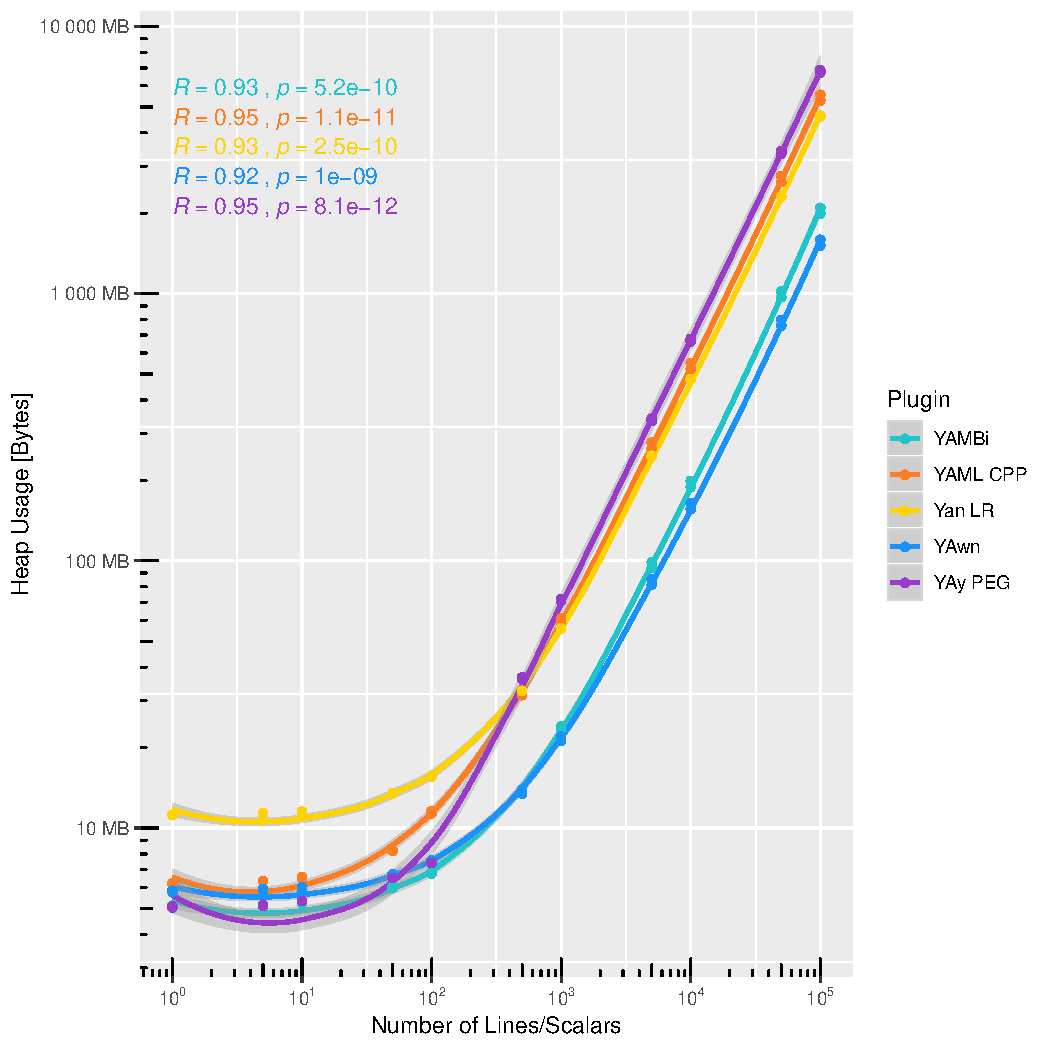
\includegraphics[width=\textwidth]{BenchmarkResultMemory}
  \caption{The diagrams above show the peak heap memory usage of the plugins for the input file \FileGeneratedHundredThousand{} and other files that contain only the first $n$ number of lines of this file.}
  \label{fig:benchmark_results_generated}
\end{figure}

\section{Error Reporting}

\emph{Error handling} can be grouped into four dependent stages~\cite{ruefenacht2016error, pottier2016reachability}:

\begin{enumerate}
  \item error detection,
  \item error diagnosis,
  \item error recovery, and
  \item error correction
\end{enumerate}

. We are mainly concerned with the first three items, since error correction is generally not possible without the possibility of fixing errors incorrectly. These errors can be disastrous in case an important configuration value, such as “radiation intensity” is set incorrectly as a result of error correction.

\emph{Error reporting} is one of the the results of

\begin{itemize}
  \item detecting that input is incorrect (error detection),
  \item finding what part of the input was incorrect (error diagnosis), and
  \item trying to resume the parsing process in case of errors (error recovery)
\end{itemize}

. While there exist techniques to enhance error reporting, by using external tools or modifying a parser engine~\cite{jeffery2003generating, cox2010errors}, we will only consider built-in solutions or slight modifications to a grammar. We do this, since extending a parser engine is out of scope of the thesis and elaborate extensions would also make the comparison concerning error reporting unfair.

\subsection{Initial Erroneous Input}

Listing \ref{lst:list_element_outside} shows the erroneous YAML data we used initially to compare the error reporting capabilities. Listing~\ref{lst:list_element_inside} and \ref{lst:list_element_removed} show two solutions to fix the problematic part of the YAML document.

\begin{listing}
  \begin{code-boxed}
    \inputminted[linenos]{yaml}{Data/Errors/list_element_outside.yaml}
  \end{code-boxed}
  \caption{The indentation of the sequence item \yaml{- element 2} is incorrect in the code above. One of the most obvious solutions to fix the syntax error would be to add a single space character right before \yaml{- element 2} (see Listing~\ref{lst:list_element_inside}). Another solution is to remove \yaml{- element 2} altogether (see Listing~\ref{lst:list_element_removed}).}
  \label{lst:list_element_outside}
\end{listing}

\begin{listing}
  \begin{code-boxed}
    \inputminted[linenos]{yaml}{Data/Correct/list_element_inside.yaml}
  \end{code-boxed}
  \caption{Usually a person would fix the error shown in Listing~\ref{lst:list_element_outside} by adding an indentation character before the sequence item \yaml{- element 2}.}
  \label{lst:list_element_inside}
\end{listing}

\begin{listing}
  \begin{code-boxed}
    \inputminted[linenos]{yaml}{Data/Correct/list_element_removed.yaml}
  \end{code-boxed}
  \caption{One of the easiest solutions to fix the code in Listing~\ref{lst:list_element_outside} for a computer program is to remove \yaml{- element 2}.}
  \label{lst:list_element_removed}
\end{listing}

\subsection{Basic Error Messages}

We started the comparison by listing the basic error messages for the YAML plugins. These messages contain the error location and the auto-generated error message by the parsing engines. For the sake of brevity we removed some uninteresting data such as the filename of the parsed file.

\begin{table}
  \caption{Basic error messages}
  \label{tab:error_messages_list_element_outside}
  \centering
  \begin{tabular}{llp{10cm}}
    \toprule
    \textbf{Plugin} & \textbf{Parser} & \textbf{Message}\\
    \midrule
    YAML CPP &
    yaml-cpp &
    yaml-cpp: error at line 3, column 1: end of map not found\\

    Yan LR &
    ANTLR &
    3:1: mismatched input \textquotesingle- \textquotesingle\ expecting BLOCK\_END\\

    YAMBi &
    Bison &
    3:1: syntax error, unexpected ELEMENT, \newline
    expecting KEY or BLOCK\_END\\

    YAwn &
    YAEP &
    3:1: Syntax error on token number 9: \newline
    “<Token, ELEMENT, -, 3:1–3:2>”\\

    YAy PEG &
    PEGTL &
    3:0(18): parse error matching tao::yaypeg::eof\\
    \bottomrule
  \end{tabular}
\end{table}

\subsubsection{Interpretation}

As we can see in Table~\ref{tab:error_messages_list_element_outside} all of the parsing engines report the error location for the code from Listing~\ref{lst:list_element_outside} correctly. The error messages also shows that the question, if the first position after a newline is at column 0 or 1, is still open for debate. Other than that we can see that YAMBi, YAML CPP, and Yan LR also show information about the expected element at the error position (end of a block \gls{collection} is missing). YAML CPP provides a better error message that also shows which type of end element is missing (end of map). This type of information can also be determined easily in all of the lexer-based parsing engine plugins (Yan LR, YAMBi, YAwn). We modified them accordingly. Table~\ref{tab:error_messages_improved_list_element_outside} shows the slightly improved error messages, highlighting the updated part of the text.

\begin{table}
  \caption{Slightly improved error messages}
  \label{tab:error_messages_improved_list_element_outside}
  \centering
  \begin{tabular}{llp{10cm}}
    \toprule
    \textbf{Plugin} & \textbf{Parser} & \textbf{Message}\\
    \midrule
    YAML CPP &
    yaml-cpp &
    yaml-cpp: error at line 3, column 1: end of map not found\\

    Yan LR &
    ANTLR &
    3:1: mismatched input \textquotesingle- \textquotesingle\ expecting \textbf{MAP\_END}\\

    YAMBi &
    Bison &
    3:1: syntax error, unexpected ELEMENT, \newline
    expecting \textbf{MAP\_END} or KEY\\

    YAwn &
    YAEP &
    3:1: Syntax error on token number 9: \newline
    “<Token, ELEMENT, -, 3:1–3:2>”\\

    YAy PEG &
    PEGTL &
    3:0(18): parse error matching tao::yaypeg::eof\\
    \bottomrule
  \end{tabular}
\end{table}

After the slight modifications to the YAML parser plugins we decided to take a closer look at the error handling capabilities of each of the parsing engines on their own in the next sections.

\subsection{ANTLR}

ANTLR uses an error listener class that provides a callback method that includes access to

\begin{itemize}
  \item the location,
  \item the offending symbol,
  \item the used recognizer class,
  \item the thrown exception, and
  \item the default error message
\end{itemize}

for each detected error. As we already saw in Table~\ref{tab:error_messages_list_element_outside}, the default error message provided by ANTLR usually describes errors already well. For the initial version of the \href{http://libelektra.org/plugins/yanlr}{Yan LR plugin}, we only stored the last error message reported by ANTLR. Since ANTLR uses methods such as token deletion and insertion to keep parsing a file, even if it contains multiple errors~\cite{parr2013definitive}, the last error message usually will not provide the the most obvious information on how to fix an error.

\begin{listing}
  \begin{minted}[autogobble, linenos]{yaml}
    key: - element 1
      - element 2 # Incorrect Indentation!
  \end{minted}
  \caption{The indentation of the sequence element \yaml{- element 2} is incorrect in the code above.}
  \label{lst:incorrect_indentation}
\end{listing}

For example, for the input shown in Listing~\ref{lst:incorrect_indentation} the parser produced the following error output:

\begin{textcode}
  2:37: extraneous input 'MAP END' expecting {STREAM_END, COMMENT}
\end{textcode}

. To fix this defect in the Yan LR plugin, we stored all error messages which resulted in the better error report:

\begin{textcode}
  2:1: mismatched input '- ' expecting MAP_END
  2:37: extraneous input 'MAP END' expecting STREAM_END
\end{textcode}

. You might also notice that in the error report \code{COMMENT} is missing from the list of expected tokens. This difference is the result of an \href{https://github.com/ElektraInitiative/libelektra/commit/0fe4953}{ambiguity in the ANTLR grammar we fixed}.

One of the more recent improvements in error messages of modern compilers such as Clang and GCC is the ability to highlight erroneous input. We also implemented this error reporting mechanism based on the Java code in \citetitle[page 158]{parr2013definitive}. The text:

\begin{textcode}
2:1: mismatched input '- ' expecting MAP_END
     - element 2 # Incorrect Indentation!
     ^^
2:37: extraneous input 'MAP END' expecting STREAM_END
      - element 2 # Incorrect Indentation!
                                          ^
\end{textcode}

shows the improved error message for Listing~\ref{lst:incorrect_indentation}. One thing that this error report still lacks is a more human friendly representation of the tokens. Someone with limited knowledge of the YAML specification and Yan LR’s lexer code will probably not know what \code{MAP\_END}, \code{MAP END} and \code{STREAM\_END} mean. One option to improve this situation is to replace the text used by the lexer (\code{MAP END}) and the parser (\code{MAP\_END}, \code{STREAM\_END}). The update of the relevant lexer code is trivial, since we can create tokens containing arbitrary text. For the parser code generated by ANLTR, we used a script that uses regular expressions to replace the relevant strings such as \cc{"MAP_END"} and \cc{"STREAM_END"}. After this update the error report for the YAML data in Listing~\ref{lst:incorrect_indentation} looks like this:

\begin{textcode}
2:1: mismatched input '- ' expecting end of map
     - element 2 # Incorrect Indentation!
     ^^
2:37: extraneous input 'end of map' expecting end of document
      - element 2 # Incorrect Indentation!
                                          ^
\end{textcode}

.

\subsection{Bison}

The first step we used to improve the error messages of the Bison parser was to define alternative names for the tokens, just like we did for Yan LR. Bison supports this feature directly, which meant we did not have to write a script to replace the symbols in the generated parser code. After this update the error message from Table~\ref{tab:error_messages_improved_list_element_outside} changed from:

\begin{textcode}
  3:1: syntax error, unexpected ELEMENT, expecting MAP_END or KEY
\end{textcode}

to

\begin{textcode}
  3:1: syntax error, unexpected element, expecting end of map or key
\end{textcode}

.

We then looked into the error recovery capabilities of Bison. Unlike ANTLR the generated parser does not do error recovery by default, but rather exits on the first error. To improve the error behavior Bison offers the possibility to add the predefined \code{error} token to a grammar. Every time the Bison parser encounters an error it will produce this token~\cite{donnelly2019bison}. We modified the grammar to allow errors inside YAML maps and sequences:

\begin{ccode}
  pairs : pair
        | pairs pair
        | pairs error /* Allow errors after key-value pairs */
        ;

  elements : element
           | elements element
           /* Allow errors after elements of a sequence */
           | elements error
           ;
\end{ccode}

. This way the parser is able to report multiple syntax errors.

\begin{listing}
  \begin{minted}[autogobble, linenos]{yaml}
    key 1: - element 1
     - element 2
    key 2: scalar
           - element 3
  \end{minted}
  \caption{The indentation of the sequence item \yaml{- element 2} is incorrect in the code above. Another error is that the value of \yaml{key 2} can not be both a scalar (\yaml{scalar}) and a sequence (containing \yaml{- element 3}).}
  \label{lst:incorrect_indentation_element_without_sequence}
\end{listing}

After the update the parser produces an error message that looks like this:

\begin{textcode}
2:2: unexpected start of sequence, expecting end of map or key
      - element 2
      ^
4:8: unexpected start of sequence, expecting end of map or key
            - element 3
            ^
\end{textcode}

the input shown in Listing~\ref{lst:incorrect_indentation_element_without_sequence}. As you can see above, we also added the erroneous input to the error message, just like we did in the Yan LR plugin.

One option to improve the error output of the Bison parser we did not implement is described by \citeauthor{jeffery2003generating} in \citetitle{jeffery2003generating}~\cite{jeffery2003generating}. The technique looks promising, and was also added to the old Bison parser\footnote{The developers of Go switched to a hand-written parser written in Go in 2016~\cite{pike2017reddit, go2016release}.} for the programming language Go~\cite{cox2010errors}. Recently \citeauthor{pottier2016reachability}~\cite{pottier2016reachability} extended \citeauthor{jeffery2003generating}’s work and added example based error reporting in the LR parsers of the CompCert C compiler~\cite{kaestner2018compcert}. In \citetitle{pottier2016reachability} \citeauthor{pottier2016reachability}~\cite{pottier2016reachability} writes:

\begin{quote}
  We believe it is fair to say that the quality of CompCert’s diagnostic messages is now on par with that of \texttt{clang} and \texttt{gcc}.
\end{quote}

. This statement and the examples in the article lead us to believe that the error messages of Yan LR could be improved using example based error reporting. However, the technique is not directly supported by Bison and hence requires changes to the parsing code that are out of the scope of this thesis.

\subsection{YAEP}

Just as Bison, YAEP also requires that you add error tokens to the grammar to specify locations for error recovery. We therefore defined the same error recovery locations inside sequences and maps, as we did with Bison. The other updates were quite similar too: We improved the name of tokens inside error messages and added the erroneous input to the error message.

After all these changes the output for the YAML data from Listing~\ref{lst:incorrect_indentation_element_without_sequence} looks very similar to the one produced by YAMBi:

\begin{textcode}
2:2: Syntax error on input “start of sequence”
      - element 2
      ^
4:8: Syntax error on input “start of sequence”
            - element 3
            ^
\end{textcode}

. The only thing missing is the information about the expected type of token.

\subsection{PEGTL}

LL and LR parsers read the input deterministically from left to right. They therefore report the first position, where the parsed input is not part of the language described by the grammar anymore. This behavior is also known as (longest) correct/viable prefix property~\cite{sippu1990parsing, ruefenacht2016error, maidl2016129, pottier2016reachability}.

\Gls{PEG} parsers do not have this property. The reason behind this is that \glspl{PEG} use backtracking, and therefore obfuscate error locations~\cite{ruefenacht2016error}. In his master thesis~\cite{ford2002packrat} \citeauthor{ford2002packrat} describes one option to produce meaningful error messages. His parser records all parsing results and uses the one that matched the farthest to the right in the input for error messages. In \citetitle{maidl2016129}~\cite{maidl2016129} \citeauthor{maidl2016129} show that this error strategy can also be added to every \gls{PEG} library that supports semantic actions. They also introduce a form of error reporting, inspired by the excepting handling mechanism of programming languages, based on grammar annotations called labeled failures~\cite{maidl2016129}.

PEGTL does neither implement the error handling strategy described by \citeauthor{ford2002packrat}~\cite{ford2002packrat}, nor labelled failures~\cite{maidl2016129}. Instead the library offers a grammar rule called \cpp{must}, which states that a certain rule, specified as template argument, has to match at a given position or an error will be raised. We can customize the code executed for a given \cpp{must} rule according to this template argument. Effectively this strategy allows us to specify different error messages for each expected but unmatched rule.

As we described in the section “\nameref{sec:peg_parser}”, we tried to keep the grammar of our PEG Parser plugin \href{https://libelektra.org/plugins/yaypeg}{YAy PEG} close to the grammar of the \href{http://yaml.org/spec/1.2/spec}{YAML specification}~\cite{ben2009yaml}. This also meant, that the grammar contained only a single \cpp{must} rule, that makes sure that the grammar matched the whole input:

\begin{cppcode}
  struct yaml : if_must<l_yaml_stream, eof> {};
\end{cppcode}

. The code above also explains the initial version of the error message shown in Table~\ref{tab:error_messages_improved_list_element_outside}:

\begin{textcode}
  3:0(18): parse error matching tao::yaypeg::eof
\end{textcode}

, which tells us, that the parser was unable to match the expected “end of file” in line 3 of the input. We customized the error message above to show a more user friendly text:

\begin{textcode}
  3:0: Incomplete document, expected “end of file”
       - element 2
       ^
\end{textcode}

. As you can see we also added the erroneous input to the message, just as we did for the other parsing engines.

The same single error message, regardless of the error, is not helpful. For good error reporting we need to add other \cpp{must} rules. However, adding failure points (\cpp{must} rules) changes the behavior of the grammar and might even cause the parser to fail on valid input. To minimize the probability of incorrect grammar changes we only added a few rules for situation we were sure that the remainder of a grammar rule had to match. For example, when the parser reads an unescaped single or double quote character (outside of a block scalar) at the beginning of a line or after a whitespace character, it found a quoted flow scalar. Therefore

\begin{enumerate}
  \item the text after the initial quote has to be followed by a (possibly empty) text containing only certain characters, and
  \item the last character of the flow scalar has to be an unescaped quote
\end{enumerate}

. If one of those two rules is not fulfilled, then the parser found a syntax error. After we updated the code accordingly the error message for the YAML data

\begin{yamlcode}
  "double quoted
\end{yamlcode}

looks like this:

\begin{textcode}
  1:14: Missing closing double quote or
        incorrect value inside flow scalar
        "double quoted
                      ^
\end{textcode}

. As you noticed we included both error possibilities in the error message, since reacting to both errors independently would require fundamental changes to the grammar.

\subsection{Final Error Messages}

\subsubsection{Element Outside of Sequence}

Table~\ref{tab:error_messages_final_list_element_outside} shows the final error messages for the code of Listing~\ref{lst:list_element_outside}:

\begin{code-boxed}
  \inputminted[linenos]{yaml}{Data/Errors/list_element_outside.yaml}
\end{code-boxed}

.

\begin{table}[H]
  \caption{Final error messages for the YAML code of Listing~\ref{lst:list_element_outside}}
  \label{tab:error_messages_final_list_element_outside}

  \centering
  \begin{tabular}{lp{0.8\textwidth}}
    \toprule
    Plugin & Error Messages\\
    \midrule

    \vspace{0cm}
    YAML CPP &
    \vspace{-0.36cm}
    \begin{textcode}
      error at line 3, column 1: end of map not found.
    \end{textcode}
    \\

    \vspace{0cm}
    Yan LR &
    \vspace{-0.36cm}
    \begin{textcode}
      3:1: mismatched input '- ' expecting end of map
           - element 2
           ^^
    \end{textcode}
    \\

    \vspace{0cm}
    YAMBi &
    \vspace{-0.36cm}
    \begin{textcode}
      3:1: syntax error, unexpected element,
           expecting end of map or key
           - element 2
           ^^
    \end{textcode}
    \\

    \vspace{0cm}
    YAwn &
    \vspace{-0.36cm}
    \begin{textcode}
      3:1: Syntax error on input “-”
           - element 2
           ^^
    \end{textcode}
    \\

    \vspace{0cm}
    YAy PEG &
    \vspace{-0.36cm}
    \begin{textcode}
      3:0: Incomplete document, expected “end of file”
           - element 2
           ^
    \end{textcode}
    \\

    \bottomrule

  \end{tabular}
\end{table}

\paragraph{Interpretation}

\begin{itemize}
  \item All the parsing engines report the correct error location.
  \item YAy PEG and YAwn do not tell us in which YAML node the error occurs. All the other plugins report that a map ended prematurely.
  \item The error message of YAMBi reports an additional option – besides deleting the input – to fix the error: adding a key (in the line between \yaml{- element 1} and \yaml{- element 2}).
\end{itemize}

The following list shows a ranking of the plugins according to the interpretation of the error messages above.

\begin{enumerate}
  \item YAMBi
  \item YAML CPP, Yan LR
  \item YAy PEG, YAwn
\end{enumerate}

\subsubsection{YAML Data Containing Multiple Errors}

The YAML data from Listing~\ref{lst:list_element_outside} only contains a single syntax error. To compare the error recovery capabilities of the parsing libraries, we used YAML data that contains multiple syntax errors as input (see Listing~\ref{lst:multiple_errors}).

\begin{listing}
  \begin{code-boxed}
    \inputminted[linenos]{yaml}{Data/Errors/multiple_errors.yaml}
  \end{code-boxed}
  \caption{The YAML data above contains three syntax errors that we directly describe in the comments right next to the error positions.}
  \label{lst:multiple_errors}
\end{listing}

Table~\ref{tab:error_messages_final_multiple_errors} shows the error messages of the different storage plugins for the YAML input of Listing~\ref{lst:multiple_errors}. As we can see the error output is quite different.

\begin{table}[H]
  \caption{Error messages for the YAML code of Listing~\ref{lst:multiple_errors}}
  \label{tab:error_messages_final_multiple_errors}
  \centering

  \begin{tabular}{lp{0.9\textwidth}}
    \toprule
    Plugin & Error Messages\\
    \midrule

    \vspace{0cm}
    YAML CPP &
    \vspace{-0.36cm}
    \begin{textcode}
      error at line 5, column 5: end of map not found.
    \end{textcode}
    \\

    \vspace{0cm}
    Yan LR &
    \vspace{-0.36cm}
    \begin{textcode}
      5:5: mismatched input 'element 3' expecting end of sequence
               element 3 # Missing `- `
               ^^^^^^^^^
      6:1: extraneous input 'end of sequence' expecting end of map
           key 3: "double quoted scalar"
           ^
      11:4: mismatched input 'start of map' expecting end of map
               key 6: # Not on same level as key 5

      13:1: mismatched input 'end of map' expecting end of document
            key 7: 'single quoted scalar'
            ^
    \end{textcode}
    \\

    \vspace{0cm}
    YAMBi &
    \vspace{-0.36cm}
    \begin{textcode}
      5:5: syntax error, unexpected plain scalar,
           expecting end of sequence or element
               element 3 # Missing `- `
               ^^^^^^^^^
      11:4: syntax error, unexpected start of map,
            expecting end of map or key
               key 6: # Not on same level as key 5
               ^
      13:1: syntax error, unexpected key, expecting end of document
            key 7: 'single quoted scalar'
            ^
    \end{textcode}
    \\

    \vspace{0cm}
    YAwn &
    \vspace{-0.36cm}
    \begin{textcode}
      5:5: Syntax error on input “element 3”
               element 3 # Missing `- `
               ^^^^^^^^^
      11:4: Syntax error on input “start of map”
               key 6: # Not on same level as key 5
               ^
      13:1: Syntax error on input “key”
            key 7: 'single quoted scalar'
            ^
      16:1: Syntax error on input “scalar”
            scalar # Not a key
            ^^^^^^
    \end{textcode}
    \\

    \vspace{0cm}
    YAy PEG &
    \vspace{-0.36cm}
    \begin{textcode}
      5:0: Incomplete document, expected “end of file”
               element 3 # Missing `- `
           ^
    \end{textcode}
    \\

    \bottomrule

  \end{tabular}

\end{table}

\paragraph{Interpretation}

\begin{itemize}

  \item \emph{YAML CPP} and \emph{YAy PEG} do not provide any error recovery.

  \item \emph{YAy PEG} shows the correct line number for the first error, but not the the correct column number. The plugin also only provides a very generic error message.

  \item All of the plugins that use error recovery (Yan LR, YAMBi, YAwn) print a spurious error messages at line 13.

  \item \emph{Yan LR} shows two error messages for the first syntax error, and one for the second syntax error. Error messages one and three describe the problematic part of the YAML data reasonably well.

  \item Compared to Yan LR, \emph{YAMBi’s} (non-spurious) error messages also describe a second option to fix the erroneous input. However, while the first error message provides a useful suggestion on how to fix the error (insertion of a sequence element), the second option in the second error messages (insertion of a key), will probably confuse anyone that does not know how YAMBi’s lexer works.

  \item \emph{YAwn} prints the same error messages as YAMBi, without the crucial information about the expected element. In addition YAwn prints a fourth error message that addresses the third syntax error.

\end{itemize}

According to the interpretation we concluded that all of the plugins with error recovery provide about the same level of useful error information. YAML CPP describes the first error reasonably well, while the error message from YAy PEG is not that useful. This leaves us with the following ranking of the error capabilities of the plugins based on the input of Listing~\ref{lst:multiple_errors}:

\begin{enumerate}
  \item Yan LR, YAMBi, Yawn
  \item YAML CPP
  \item YAy PEG
\end{enumerate}

.

\subsubsection{Conclusion}

While the parsing libraries do not produce particularly great error messages, at least the ANTLR (Yan LR) and Bison (YAMBi) plugin, provide error messages that are comparable in quality to the ones of the handwritten parsing engine (YAML CPP).

One advantage of Yan LR, YAMBi, and YAwn is that their parsers offer error recovery. They are therefore able to report multiple errors in a file. This is something that YAML CPP is currently not able to do. ANTLR offers error recovery for free, while Bison and YAEP require us to add error tokens to the grammar. This can be problematic, since these error tokens can produce conflicts in the case of Bison, and ambiguous parsing results in the case of YAEP.

The parsing plugin that showed the least useful error messages is YAy PEG. While the PEGTL offers basic error handling facilities that are able to provide good error messages for character level errors, producing good error messages for “high-level” errors would probably require a substantial amount of work.
